\def\CC{{C\nolinebreak[4]\hspace{-.05em}\raisebox{.4ex}{\tiny\bf ++}}}


\begin{frame}\frametitle{Outline}
\begin{itemize}
\item What is Pyrometheus, and what does it do
\item How is Pyrometheus used in MIRGE-Com
\item Pyrometheus software integration into MIRGE-Com
\item MIRGE-Com performance for mixtures
\item Wrap-up
\end{itemize}
\end{frame}

\begin{frame}\frametitle{Integrating \textit{Prometheus} into \textit{mirgecom}}
There are 4 \textit{Prometheus} constructs to consider for integration:
\begin{itemize}
\item Mechanism generation
\item Equation of state (EOS)
\item Chemistry
\item ``Advanced'' transport (future)
\end{itemize}
\end{frame}

\begin{frame}\frametitle{\textit{Prometheus} mechanism code generation}
\begin{multicols}{2}
\begin{itemize}
   \item \plusplus{C} command-line utility (is not Python)
   \item XML $\rightarrow$ \textit{Prometheus}(\textit{Cantera}) $\rightarrow$ Python interface for EOS, chemistry, (\& transport)
\end{itemize}
\begin{itemize}
   \item Integration options:
   \begin{itemize}
      \item Full integration - \textit{mirgecom} ingests XML, uses \textit{Prometheus} to generate mechanism, including mechanism in \textit{mirgecom} library
      \item Partial integration - \textit{Prometheus} pre-generates mechanism for inclusion of interface into \textit{mirgecom} library
      \item Non-integration - \textit{Prometheus} stand-alone library implements one or more mechanisms and is used as a substrate library by \textit{mirgecom} 
   \end{itemize}
    \item Staged integration - partial $\rightarrow$ full
   \item Tests we can do right away (regardless of integration level):
   \begin{itemize}
      \item Pre-generated mechanism Python code inclusion (\textit{mirgecom} build and run)
      \item Pre-generated mechanism function invocations (smoke tests \& screening)
   \end{itemize}
\end{itemize}
\end{multicols}
\end{frame}

\begin{frame}\frametitle{\textit{Prometheus} EOS}
\begin{multicols}{2}
\begin{itemize}
   \item Interface functions
   \begin{itemize}
      \item get\_temperature(e, Y, Tguess) $\rightarrow (T, Cp_{mix}, R_{mix})$
      \item get\_pressure(Y, T) $\rightarrow P_{mix}$ 
      \item get\_mix\_cp(T, Y) $\rightarrow (Cp_{mix})$ 
      \item get\_mix\_cv(T, Y) $\rightarrow (Cv_{mix})$
      \item get\_mix\_e(T, Y) $\rightarrow (e)$
      \item get\_mix\_enthalpy(T, Y) $\rightarrow (h_{mix})$
      \item get\_species\_cp\_R(T) $\rightarrow (Cp_{i})$ 
      \item get\_species\_enthalpies(T, Y) $\rightarrow (h_{i})$
   \end{itemize}
   \item Wrap interface to \textit{mirgecom} standard EOS - small to medium effort
   \item Special considerations
   \begin{itemize}
      \item Species ordering, naming
      \item Buffer species handling
   \end{itemize}
   \item Potential tests:
   \begin{itemize}
     \item Species-specific mixture tests (i.e. one species-at-a-time)
     \item Calorically perfect mixture - Compare Prometheus vs. \textit{mirgecom}@CPEOS
     \item Thermally perfect mixture with linear $Cp_i$ - test temperature inversion vs. analytic? 
   \end{itemize}
\end{itemize}
\end{multicols}
\end{frame}

\begin{frame}\frametitle{Wrappers for \textit{Prometheus} EOS}
Create \textit{mirgecom}-EOS-compatible wrappers for \textit{Prometheus} interface functions.
\begin{itemize}
\item get\_pressure(state)
\item get\_temperature(state)
\item get\_internal\_energy(state)
\item get\_speed\_of\_sound(state)
\end{itemize}
\end{frame}

\begin{frame}\frametitle{\textit{Prometheus} chemistry \& transport}
\begin{itemize}
\item Chemistry - get\_net\_production\_rates($\rho$, T, Y) $\rightarrow (\dot{\omega}_i)$
\item For explicit integration - directly feeds species source terms $S_i = (W_i \dot{\omega}_i)$
\item Transport
   \begin{itemize}
      \item Species:  $(\kappa_i, \mu_i, D_{ij})$
      \item Mixture: $(\kappa, \mu, D_i)$
   \end{itemize}
\end{itemize}
%\end{multicols}
\end{frame}

\begin{frame}\frametitle{\textit{Prometheus} / \textit{mirgecom} wishlist}
\begin{itemize}
   \item get\_species\_index(species\_name) - useful for coding the interface/wrappers
   \item get\_species\_names - for I/O, viz/analysis
\end{itemize}           
\end{frame}


% \begin{frame}\frametitle{MIRGE Overview}
% 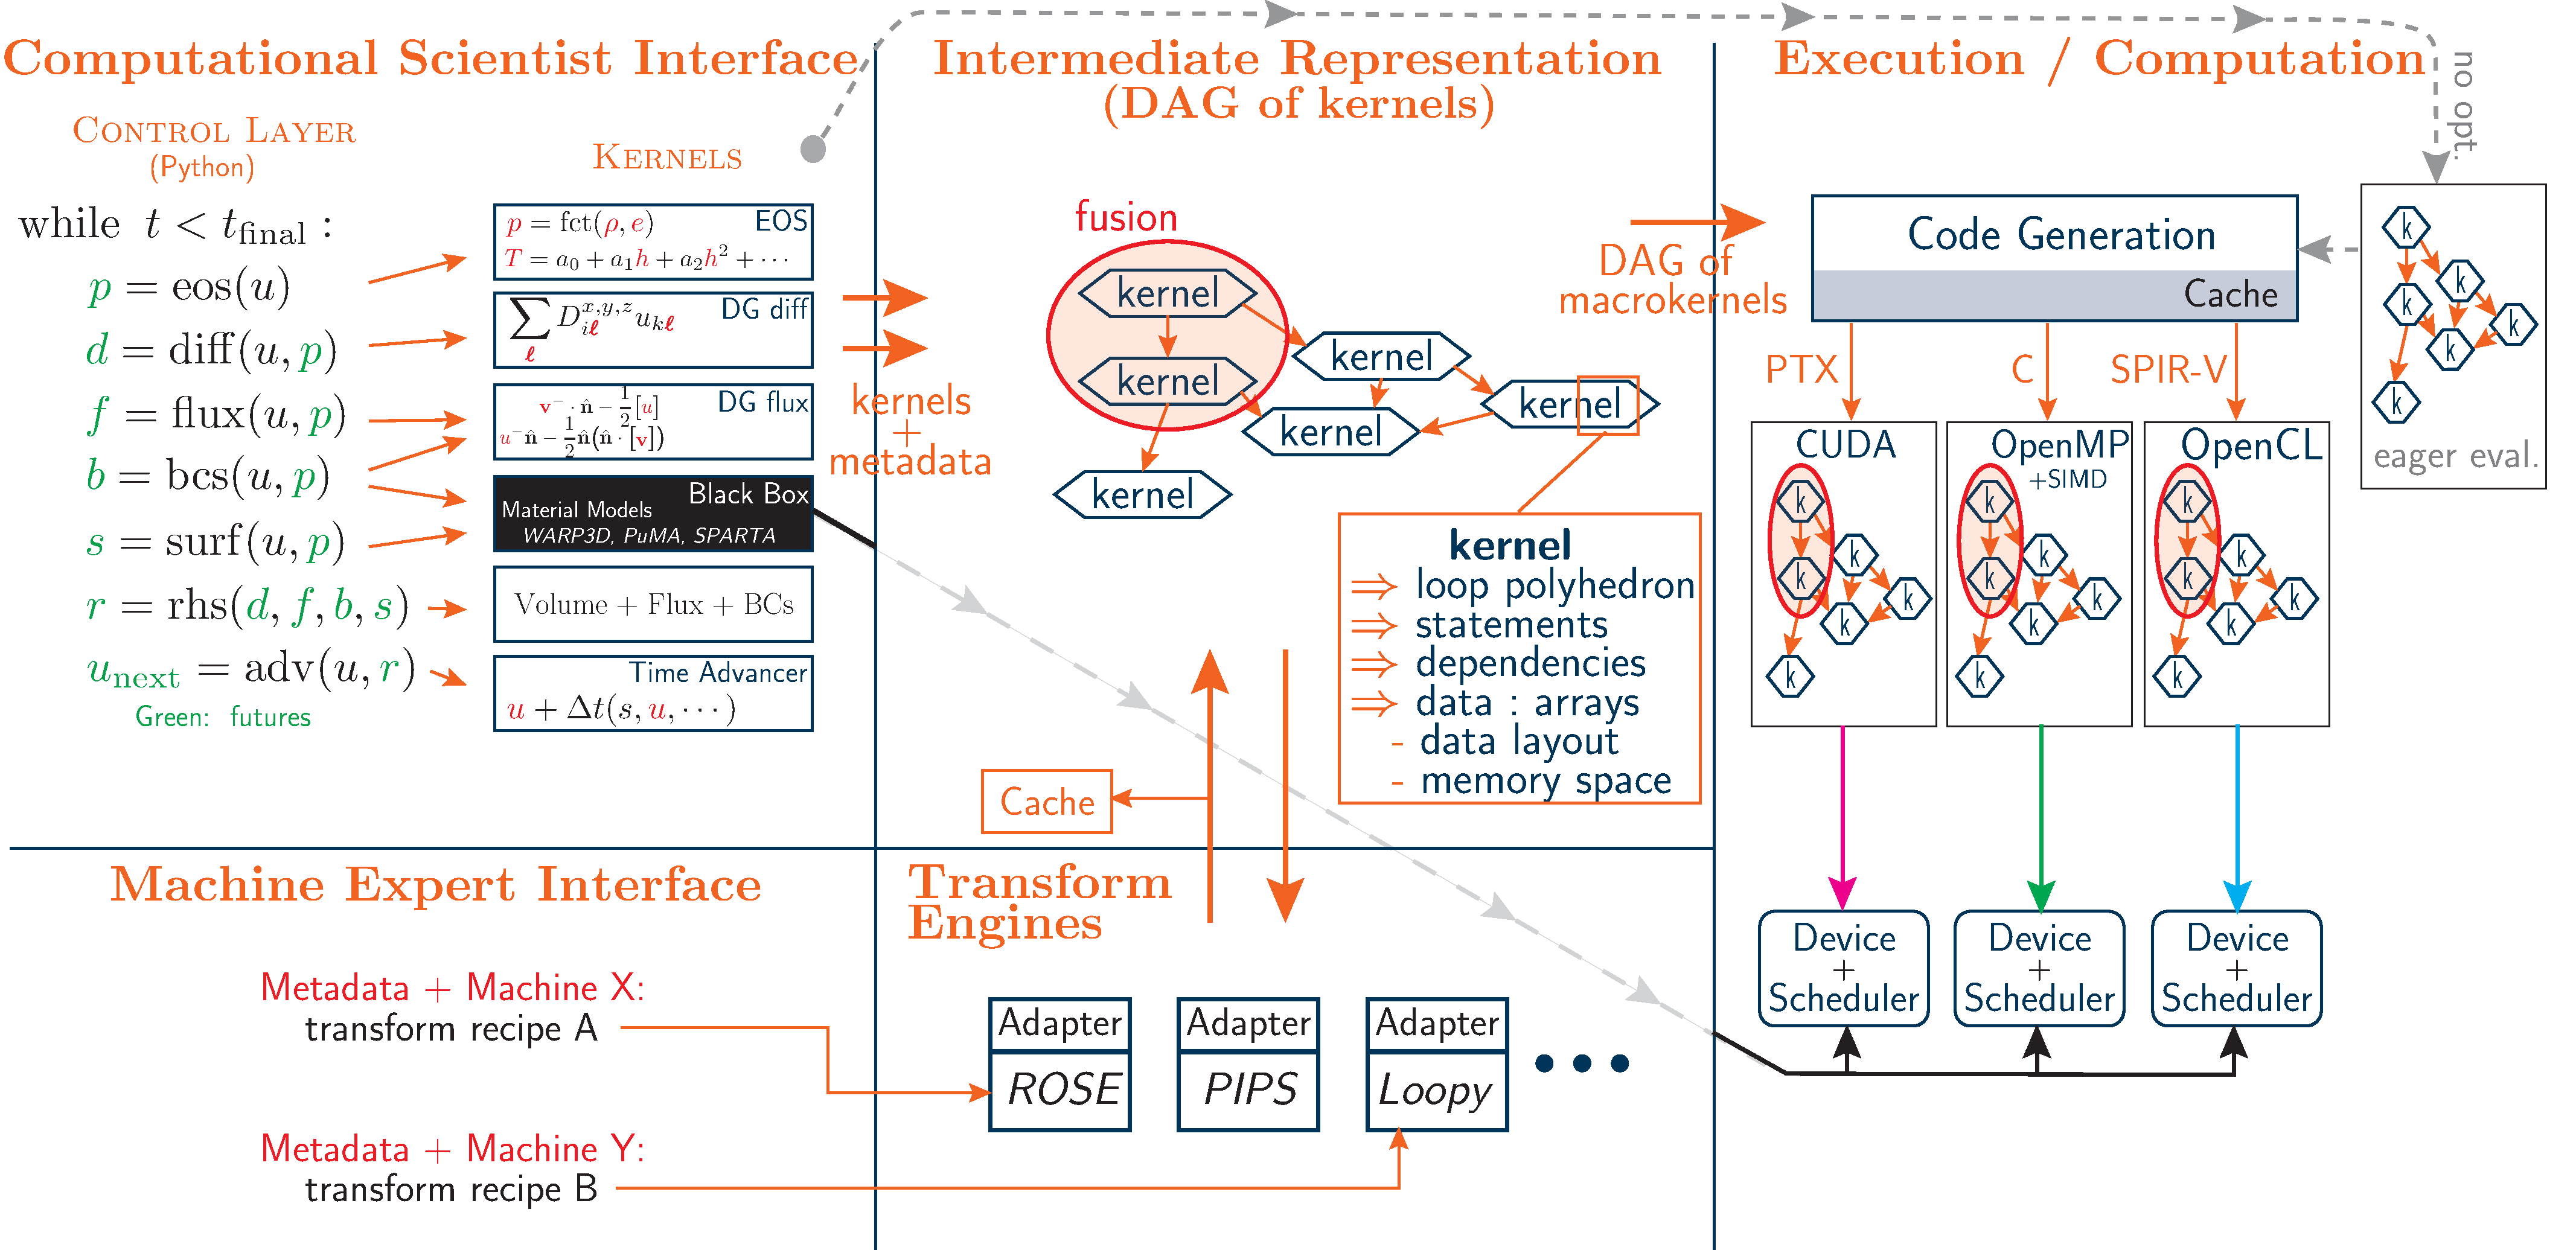
\includegraphics[width=\textwidth]{../01-Overview/figures/controllayer-new.pdf}
% \end{frame}




\begin{frame}\frametitle{\textit{MIRGE-Com} use case: Euler flow solver}
  \begin{center}
    Evolution equation:
    \begin{equation*}
      \frac{\partial\mathbf{Q}}{\partial{t}} = \mathbf{S} - (\nabla \cdot \mathbf{F}) 
    \end{equation*}
    Where state vector $\mathbf{Q}$, inviscid fluxes $\mathbf{F}$ , and sources $\mathbf{S}$ are given by:
    \begin{equation*}
      \mathbf{Q} = \begin{bmatrix}
        \rho\\\rho{E}\\\rho\vec{v}\\\rho{Y}_\alpha\end{bmatrix},\quad
      \mathbf{F} = \begin{bmatrix} \rho\vec{v}\\(\rho{E} +
        p)\vec{v}\\\rho(\vec{v} \otimes \vec{v}) +
        p\delta_{ij}\\\rho{Y}_\alpha\vec{v}\end{bmatrix}, \quad \mathbf{S} = \begin{bmatrix} s_\rho\\s_e\\s_{\vec{p}}\\s_{\alpha}\end{bmatrix}
    \end{equation*}
    With some equation of state (EOS) $\rightarrow~~(p,T,e)(\mathbf{Q})$
  \end{center}
\end{frame}


% AK-sanctioned rip-off 
% \begin{frame}\frametitle{DG - The program}
%   \begin{multicols}{2}
%     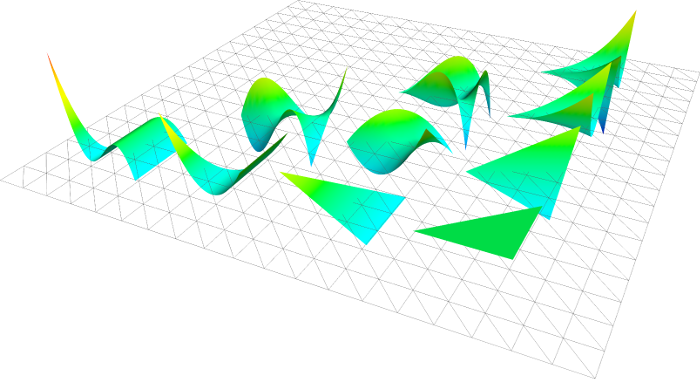
\includegraphics[width=0.4\textwidth]{../02-CS/Figures/pkdo-2d.png}
%     \vspace{-10pt}
%    \newcommand{\meshnodes}{
  \coordinate (a) at (4.53,2.86) ;
  \coordinate (b) at (2.91,3.55) ;
  \coordinate (c) at (2.25,1.8) ;
  \coordinate (d) at (-0.3,3.25) ;
  \coordinate (e) at (1.31,4.17) ;
  \coordinate (f) at (1.19,0.43) ;
  \coordinate (g) at (2.77,0.7) ;
  \coordinate (h) at (3.96,3.54) ;
  \coordinate (i) at (0.05,1.17) ;
  \coordinate (j) at (2,3.1) ;
  \coordinate (k) at (3,4.7) ;
  \coordinate (m) at (3.93,1.65) ;
  \coordinate (n) at (1.78,0.76) ;
  \coordinate (o) at (0.40,4.4) ;
  \coordinate (p) at (0.8,2.5) ;
  \coordinate (q) at (4.72,1.32) ;
  \coordinate (r) at (3.02,2.27) ;
  \coordinate (s) at (0.98,1.83) ;
  \coordinate (t) at (-0.3,1.8) ;
}


\newcommand{\withmeshtris}[1]{
  #1 cgn #1 snf #1 jsc #1 pjs
  #1 pts #1 sif #1 sit #1 dtp
  #1 odp #1 epj #1 jcb #1 oep
  #1 rcg #1 crb #1 kbh #1 rah
  #1 ejb #1 rgm #1 ram #1 qam
  #1 ekb #1 gqm #1 scn #1 bhr
}

\newcommand{\drawtriangle}[3]
  {\draw (#1) -- (#2) -- (#3) -- cycle;}
\newcommand{\meshtris}{
  \withmeshtris\drawtriangle
}
\def\drawnodenames{
  \foreach \i in {a,b,c,d,e,f,g,h,i,j,k,m,n,o,p,q,r,s,t}
    \node at (\i) {\i};
}
  

%     \begin{tikzpicture}[scale=0.4]
%       \meshnodes
%       \meshtris
%       \draw [fill=blue!30] (c) -- (n) -- (g) ;
%       \node [left=10mm of g,xshift=-2mm] (ellabel) {$E_k$};
%       \draw [thick,->,shorten >=2mm] (ellabel) -- (c) ;
%     \end{tikzpicture}
%     \vspace{-10pt}
%     \prj{\tiny}{Kl{\"o}ckner}\columnbreak \\
%     Numerical approximation to $\mathbf{Q}$, $\mathbf{S}$:
%     \begin{equation*}
%       \partial_t\mathbf{q}^{*} + \nabla \cdot \mathbf{F}(\mathbf{q}^{*}) - \mathbf{s}^{*} = 0
%     \end{equation*}
%     Hit with test function and integrate over element:
%     \begin{equation*}
%       \int_{E_k}[(\partial_t\mathbf{q}^{*} - \mathbf{s}^{*}) + (\nabla \cdot \mathbf{F}(\mathbf{q}^{*}))]\phi\,dx = 0
%     \end{equation*}
%   \end{multicols}
 %  \begin{center}
%     Integrate by parts:
%     \begin{equation*}
%       \int_{E_k}(\partial_t\mathbf{q}^{*}- \mathbf{s}^{*})\phi\,dx -
%       \int_{E_k}(\mathbf{F}(\mathbf{q}^{*}) \cdot \nabla{\phi})\,dx +
%       \int_{\partial{E_k}}(\hat{n} \cdot \mathbf{F}(\mathbf{q}^{*}))\phi\,dx
%     \end{equation*}
 %  \end{center}
%   \begin{center}
%     Rearranging in matrix form:
%     \begin{equation*}
%       \mathcal{M}[\partial_t\mathbf{q}^{*}] = \mathcal{M}[\mathbf{s}^{*}] + ( \mathcal{S}[\mathbf{F}(\mathbf{q}^{*})] )
%       - \sum{\mathcal{M}_{\partial{E_k}}[(\hat{\mathbf{n}} \cdot \mathbf{f}^{*})]} ) 
%     \end{equation*}
%   \end{center}
% \end{frame}


\begin{frame}\frametitle{Euler RHS}
\begin{multicols}{2}
\begin{itemize}
  \item \textit{Grudge} provides:
  \begin{itemize}
    \item weak div operator, ($\mathcal{S}$)
    \item boundary traces % interior\_trace\_pair - selects all interior faces
      %    \item cross\_rank\_trace\_pairs - selects all partition boundary pairs
    \item mass matrix ($\mathcal{M}^{\neg 1}$)
  \end{itemize}
  \item Euler provides: fluxes $\mathbf{F}, \mathbf{f}^{*}$
  \item User provides:
  \begin{itemize}
  \item state \& sources \textbf{Q}, \textbf{S}
  \item EOS (pressure)
  \item boundaries
  \end{itemize}
\end{itemize}
\end{multicols}
% \lstinputlisting[style=kkcodestyle, basicstyle=\tiny, language=Python]{figures/mtc/rhs_sample.py}
%\begin{multicols}{2}
%  \lstinputlisting[style=kkcodestyle, basicstyle=\tiny, language=Python]{figures/mtc/rhs_sample2.py}
%\columnbreak
%  \lstinputlisting[style=kkcodestyle, basicstyle=\tiny, language=Python]{figures/mtc/rhs_sample3.py}
%\end{multicols}
\end{frame}

\begin{frame}\frametitle{Example Euler simulation applications}
\begin{multicols}{2}
  \begin{itemize}
  \item CI-exercised verification cases 
    \begin{itemize}
    \item Isentropic vortex
    \item Sod's shock
    \item Scalar advection
    \end{itemize}
  \item More simulation support stuff
    \begin{itemize}
    \item Grid gen/decomp (serial)
    \item Generic time marching
    \item RK4 time integrator 
    \item Viz I/O - VTK file/process
    \item Status \& profiling \prj{\tiny}{M.~Diener}
    \end{itemize}
\end{itemize}
\end{multicols}
\begin{center}
  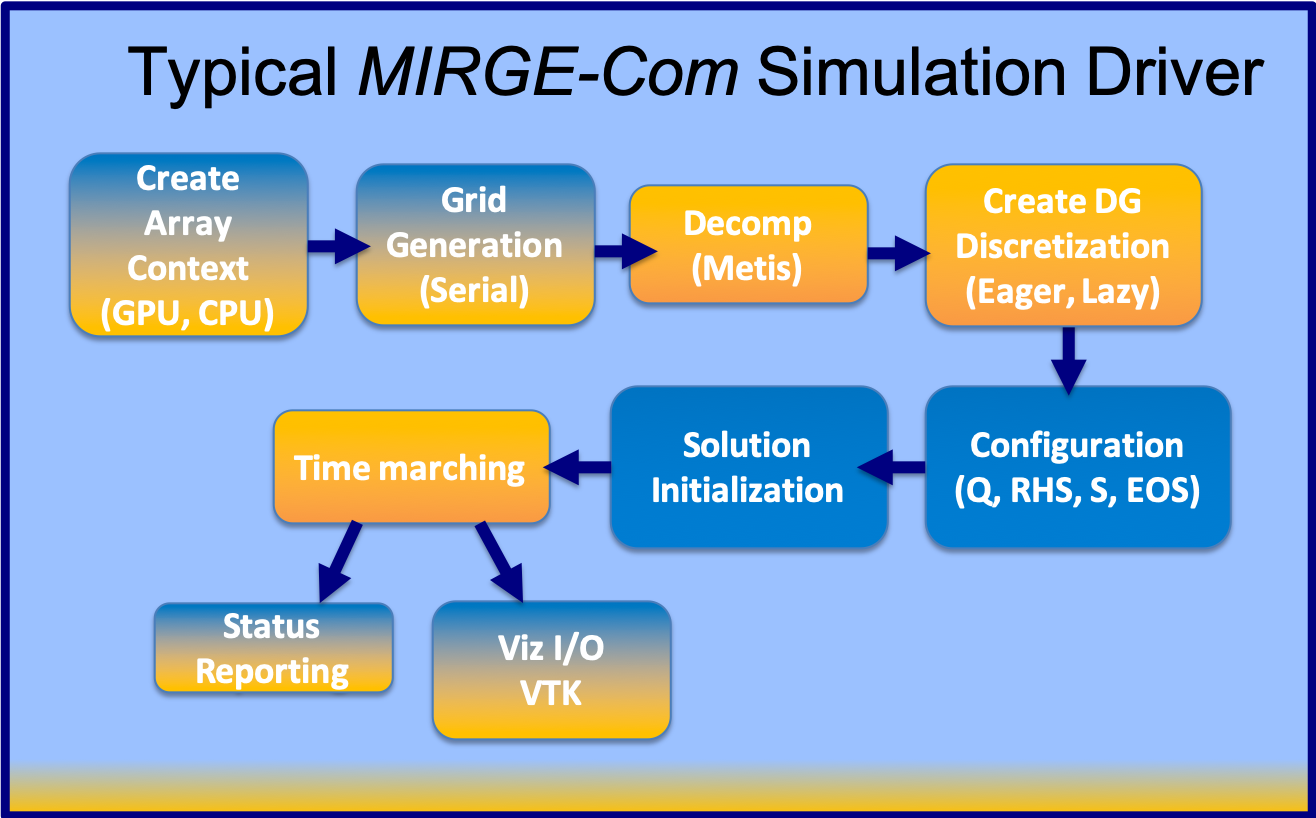
\includegraphics[width=.7\textwidth]{figures/mtc/TypicalDriver2.png}
\end{center}
\end{frame}

%\begin{frame}\frametitle{Example Euler simulation applications}
%\begin{multicols}{2}
%  \begin{itemize}
%  \item CI-exercised verification cases 
%    \begin{itemize}
%    \item Isentropic vortex
%    \item Sod's shock
%    \item Scalar advection
%    \end{itemize}
%  \item More simulation support stuff
%    \begin{itemize}
%    \item Grid gen/decomp (serial)
%    \item Generic time marching
%    \item RK4 time integrator 
%    \item Viz I/O - VTK file/process
%    \item Status \& profiling \prj{\tiny}{M.~Diener}
%    \end{itemize}
%\end{itemize}
%\end{multicols}
%\begin{multicols}{2}
%  \lstinputlisting[style=kkcodestyle, basicstyle=\tiny, language=Python]{figures/mtc/vortex_driver.py}
%  \lstinputlisting[style=kkcodestyle, basicstyle=\tiny, language=Python]{figures/mtc/vortex_driver1.py}
%  \columnbreak
%  \lstinputlisting[style=kkcodestyle, basicstyle=\tiny, language=Python]{figures/mtc/vortex_driver2.py}
%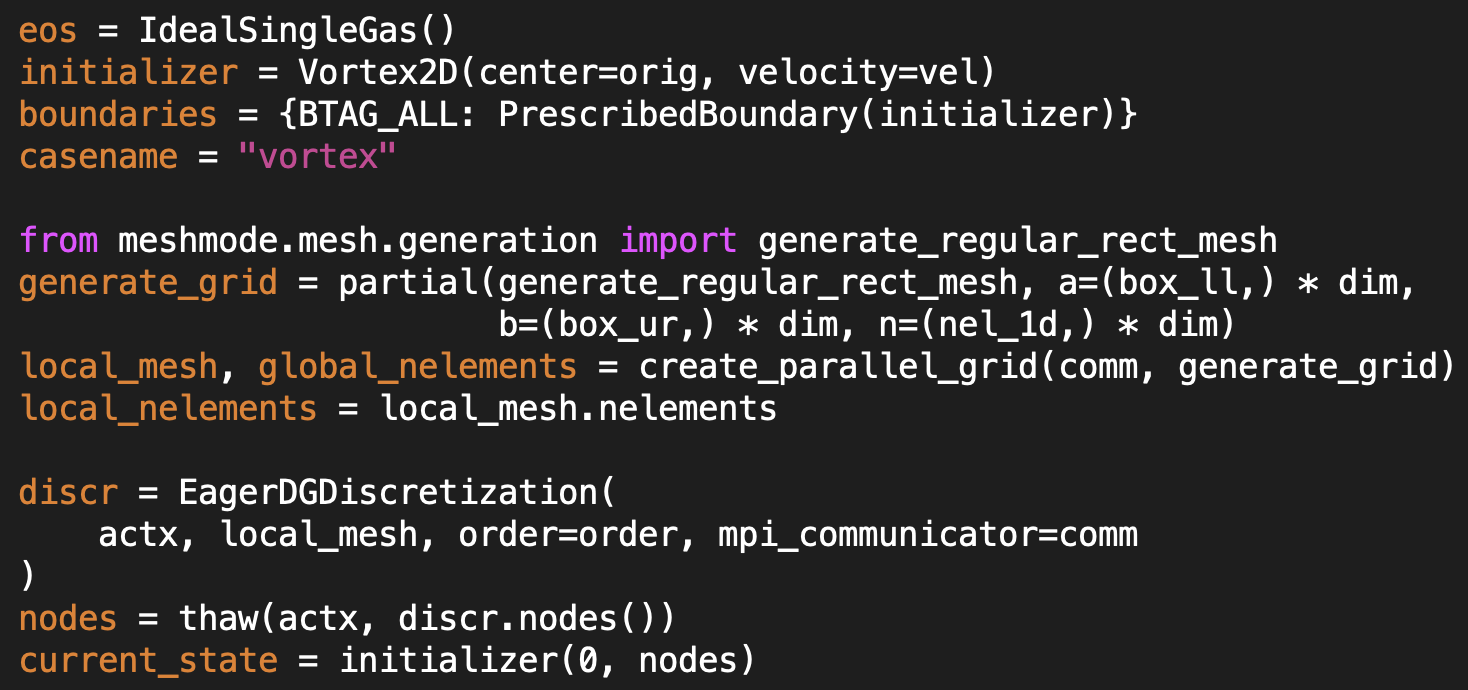
\includegraphics[width=.45\textwidth]{figures/mtc/vortex_driver1.py}
%\hspace{.2in}
%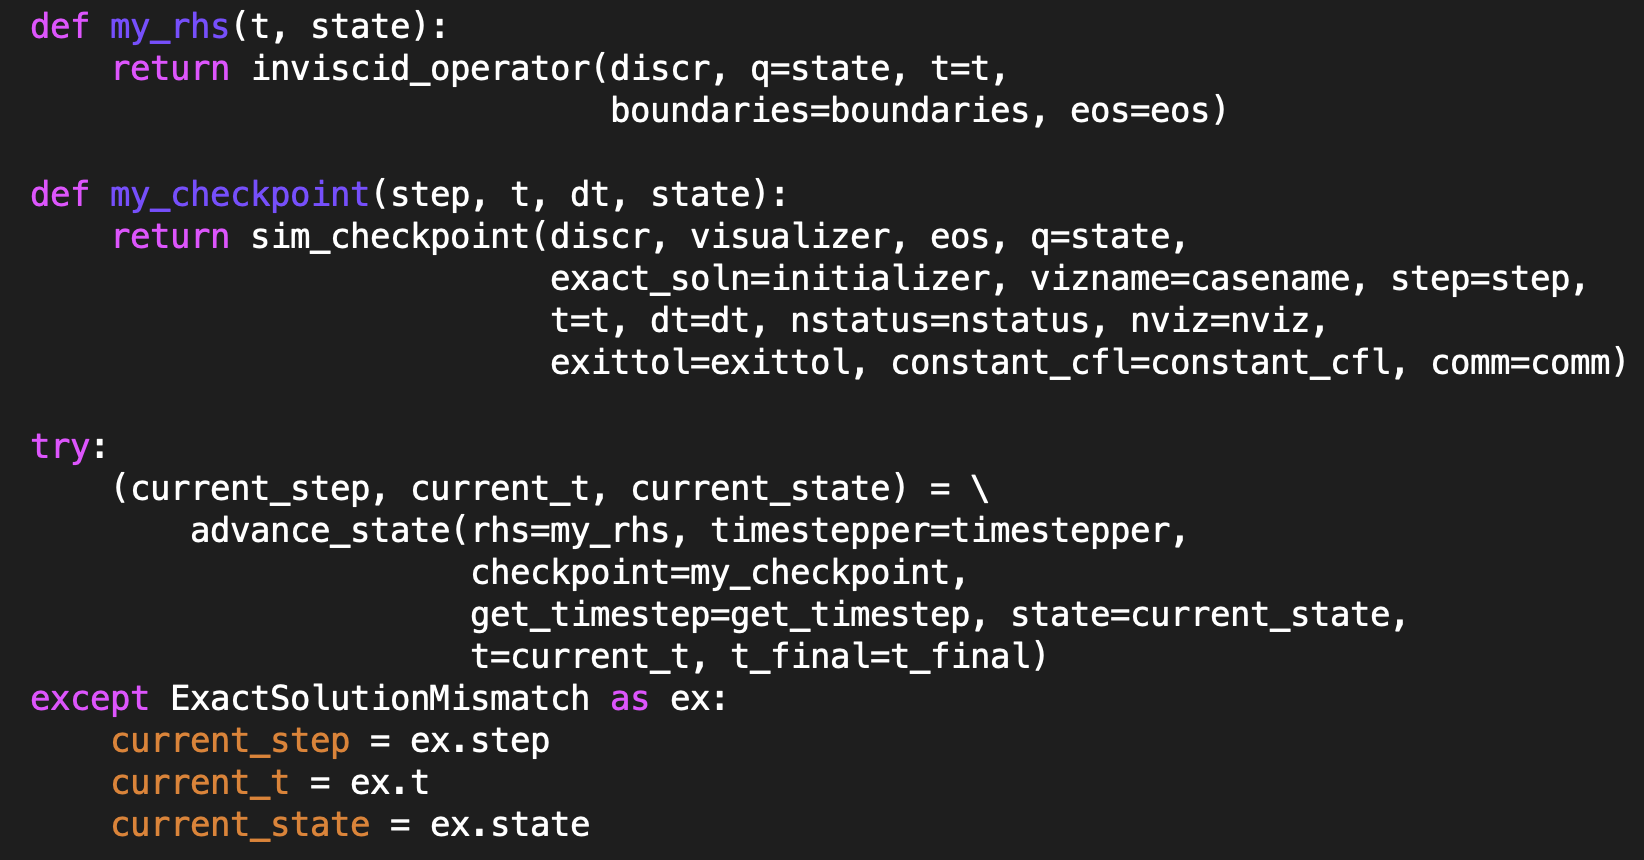
\includegraphics[width=.45\textwidth]{figures/mtc/vortex_driver2.py}
%\end{multicols}
%\end{frame}

\begin{frame}\frametitle{Mixtures with \textit{MIRGE-Euler}}
  \begin{center}
  Goal: Add reactive mixture mechanisms to \mirgecom{}\\
  Plan: Use \textit{Prometheus} / \textit{Pyrometheus}\\
  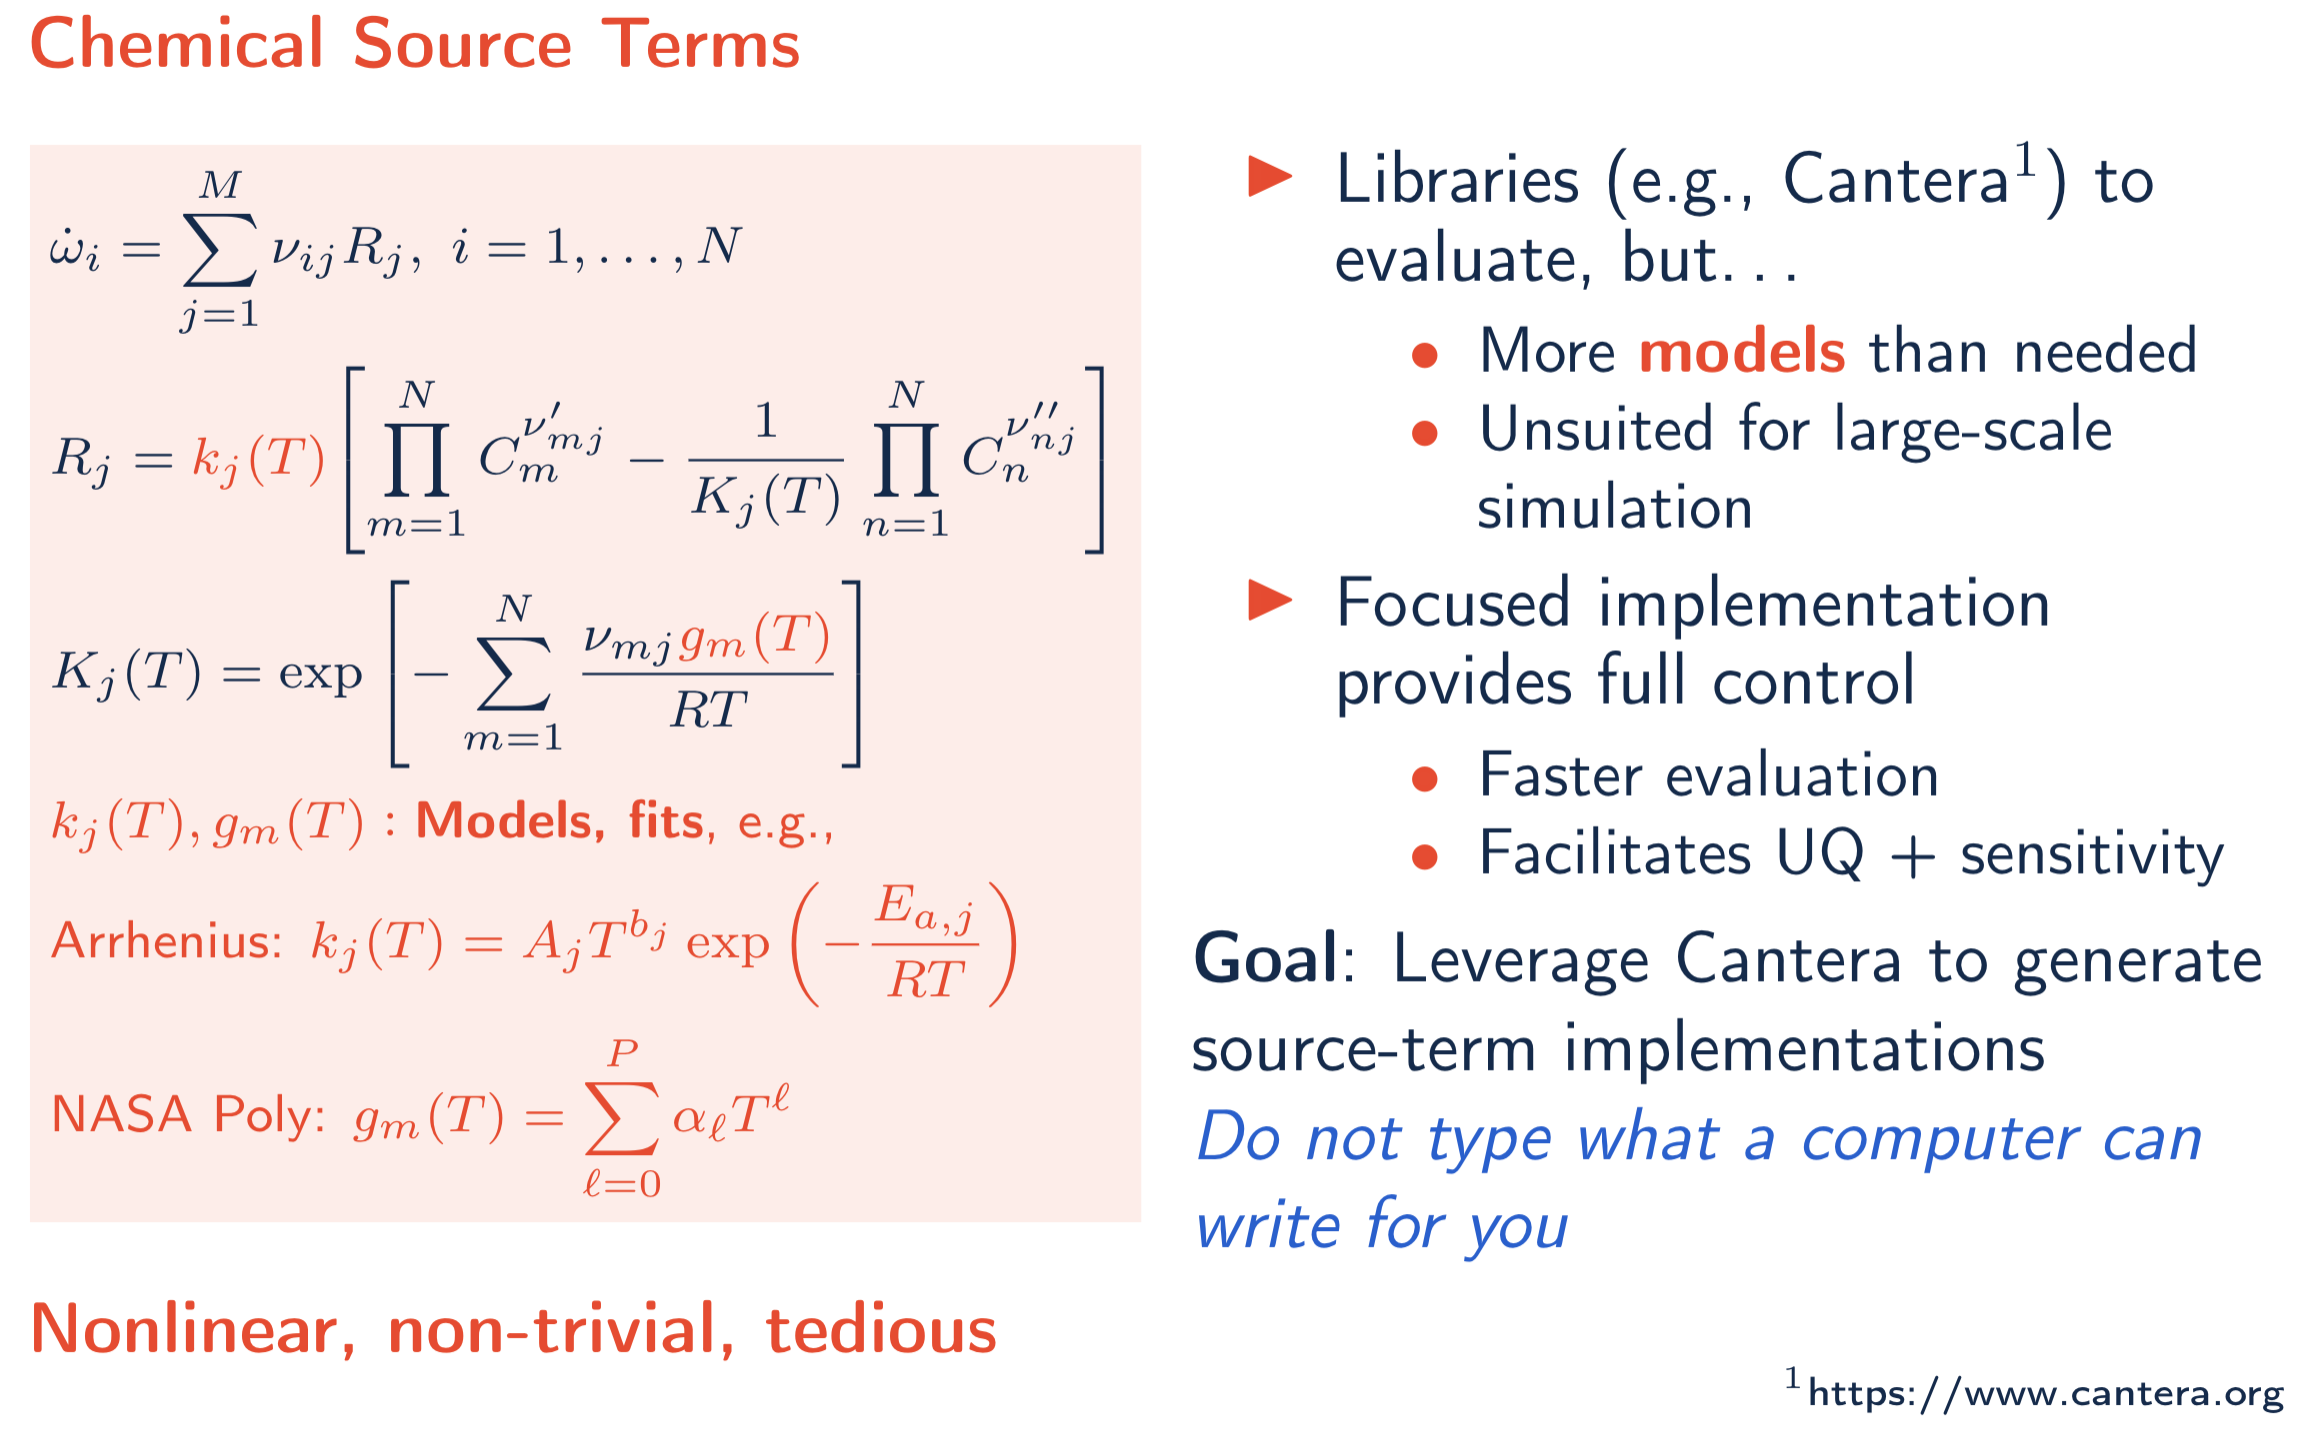
\includegraphics[width=.8\textwidth]{figures/mtc/Prometheus1.png}
  \\
 \prj{\tiny}{Esteban Cisneros}
  \end{center}
\end{frame}

\begin{frame}\frametitle{\textit{Prometheus} $\rightarrow$ \textit{Pyrometheus}}
  \begin{multicols}{2}
%    \begin{itemize}
%    \item \textit{Prometheus}
      \begin{itemize}
      \item ThermoChemistry source generator (C\plusplus{})
      \item Uses \textit{Cantera} and generates C\plusplus{} or Python
      \end{itemize}
      \columnbreak
%    \item \textit{Pyrometheus}
      \begin{itemize}
      \item Generator port to Python (inline)
      \item Vectorize + \textit{MIRGE}-compatible
      \item \textit{MIRGE-Euler} EOS
      \end{itemize}
%    \end{itemize}
  \end{multicols}
%  \vspace{-15pt}
  \begin{multicols}{2}
    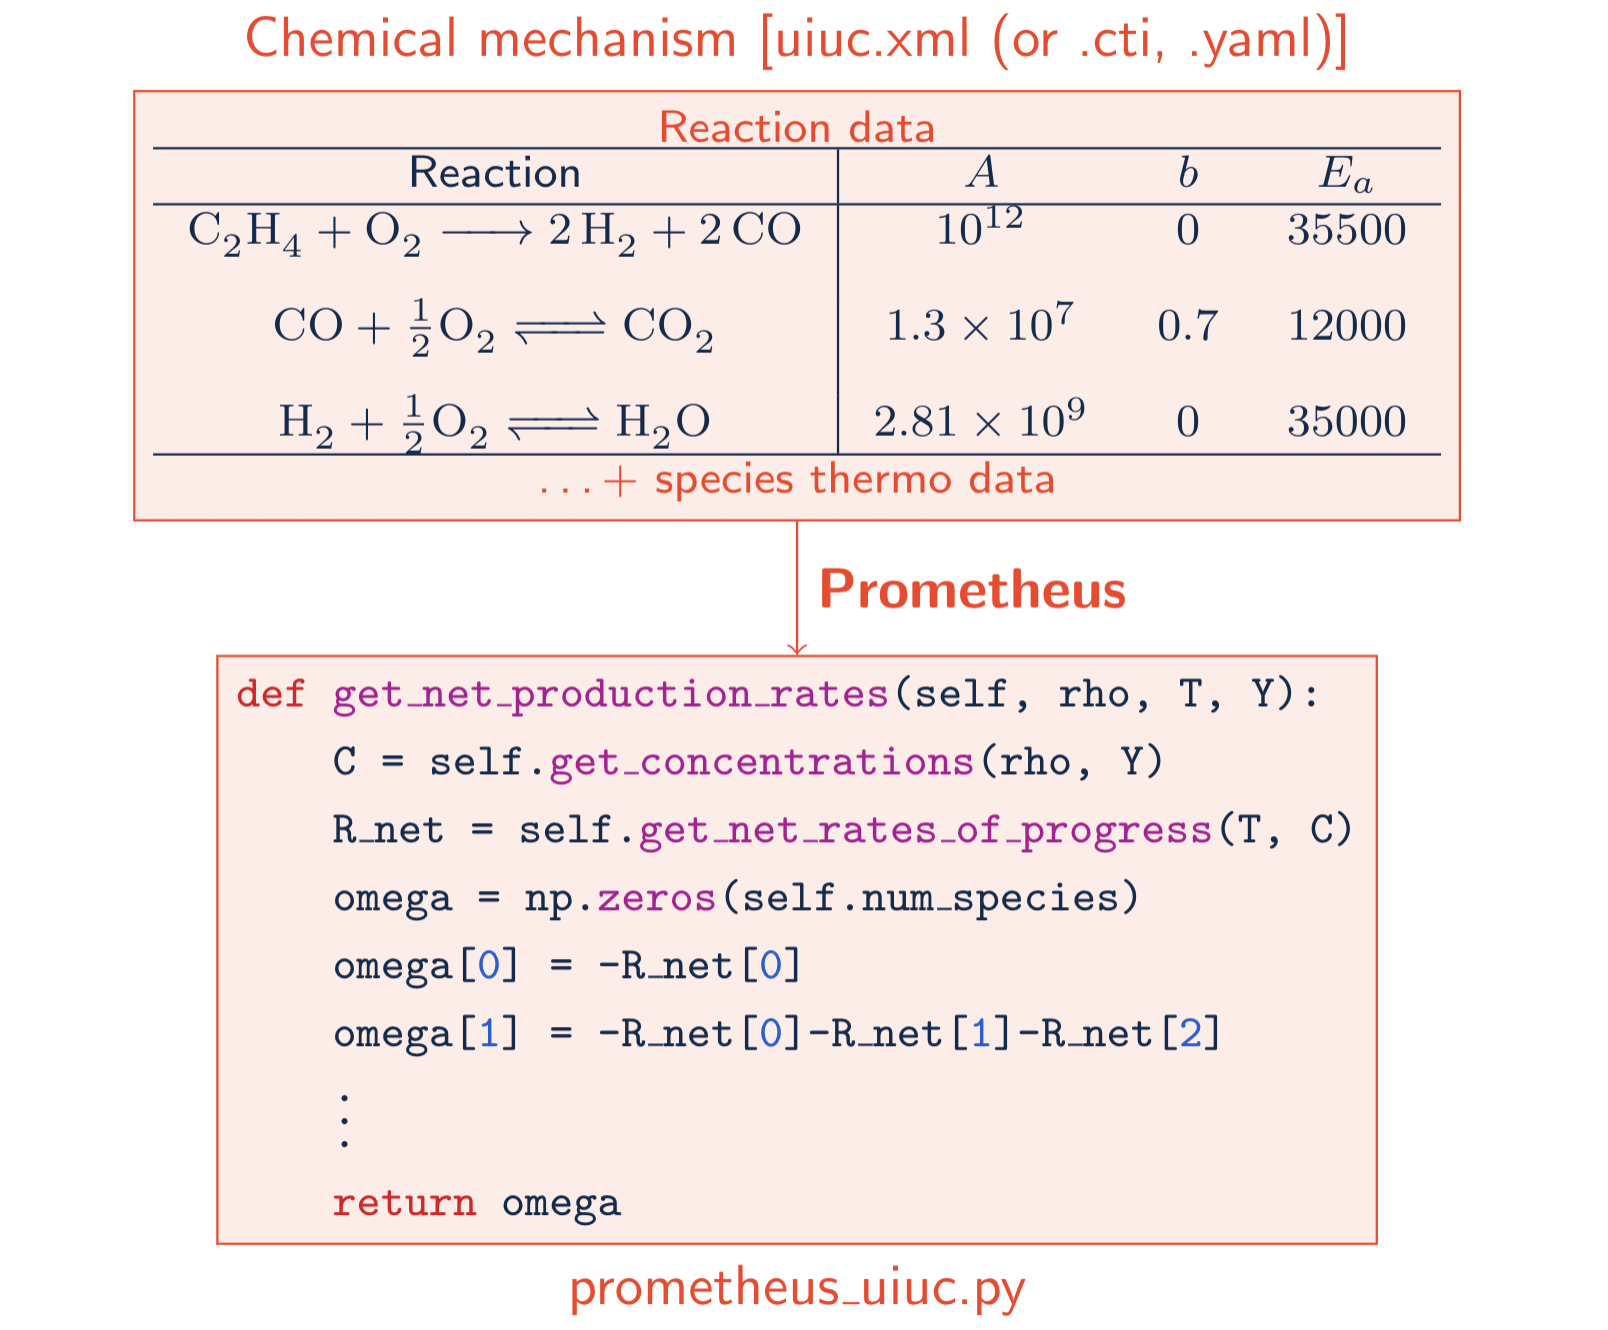
\includegraphics[width=.5\textwidth]{figures/mtc/Prometheus2.png}\\
    \begin{center}
      \prj{\tiny}{Esteban Cisneros}
    \end{center}
      \columnbreak
      \vspace{10pt}
    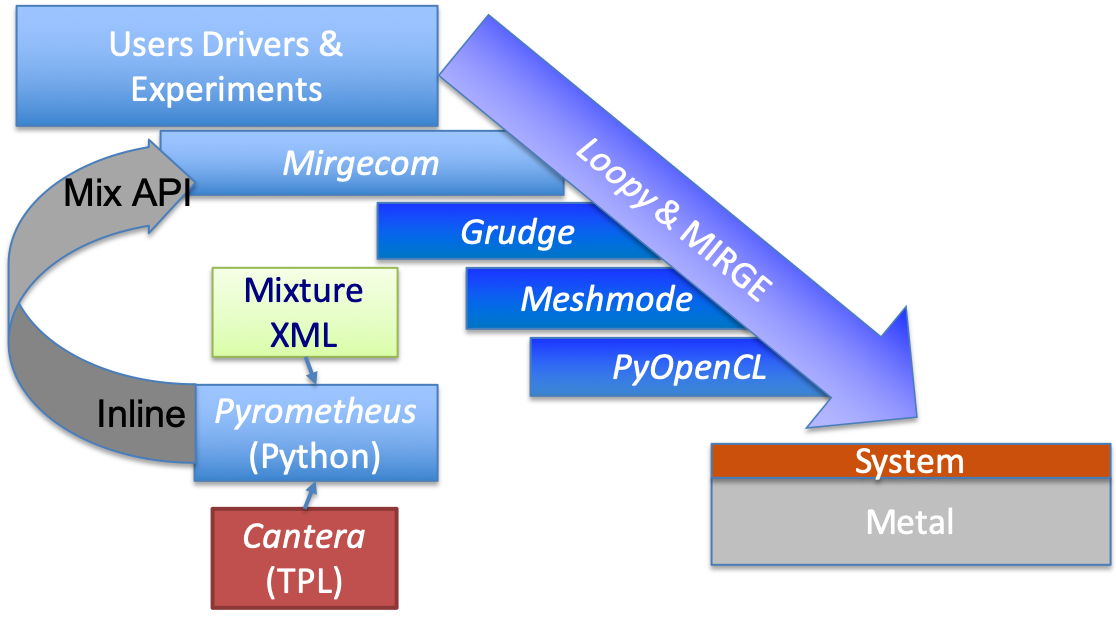
\includegraphics[width=.5\textwidth]{figures/mtc/PyrometheusIntegration.png}    
  \end{multicols}
\end{frame}

%\begin{frame}\frametitle{\textit{Pyrometheus} integration with \textit{MIRGE-Euler}}
%    \begin{multicols}{2}
%    \begin{itemize}
%    \item Port \textit{Prometheus} generator to Python $\rightarrow$ \textit{Pyrometheus}
%    \item Massage interface for MIRGE paradigm
%    \item Implement EOS and Chem Source
%    \end{itemize}
%    \end{multicols}
%    \begin{multicols}{2}
%      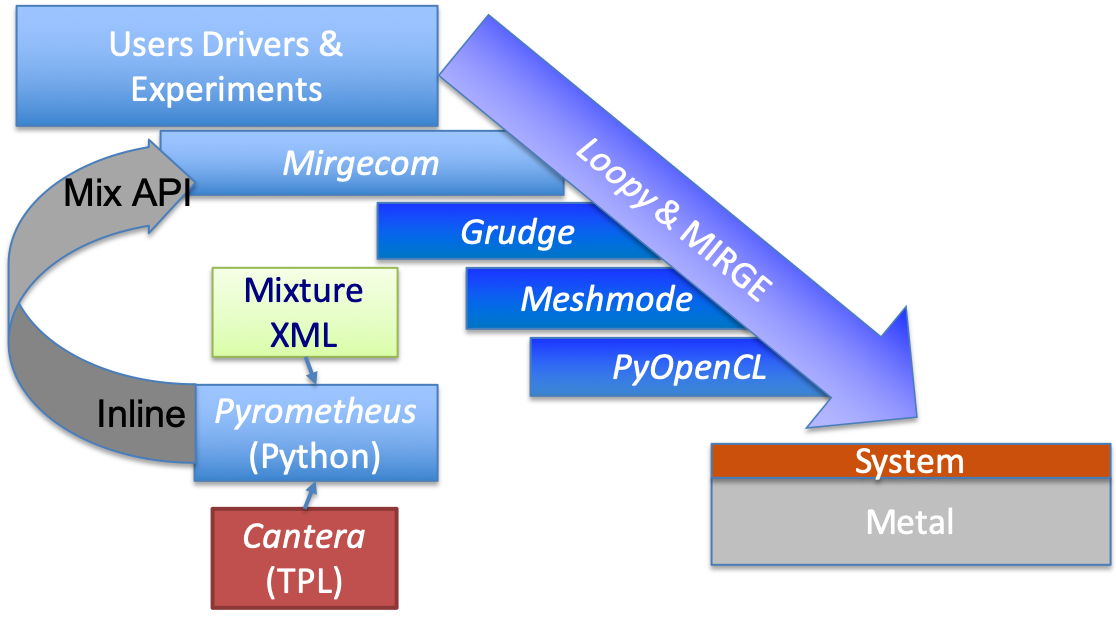
\includegraphics[width=.5\textwidth]{figures/mtc/PyrometheusIntegration.png}\\
%      \columnbreak
%      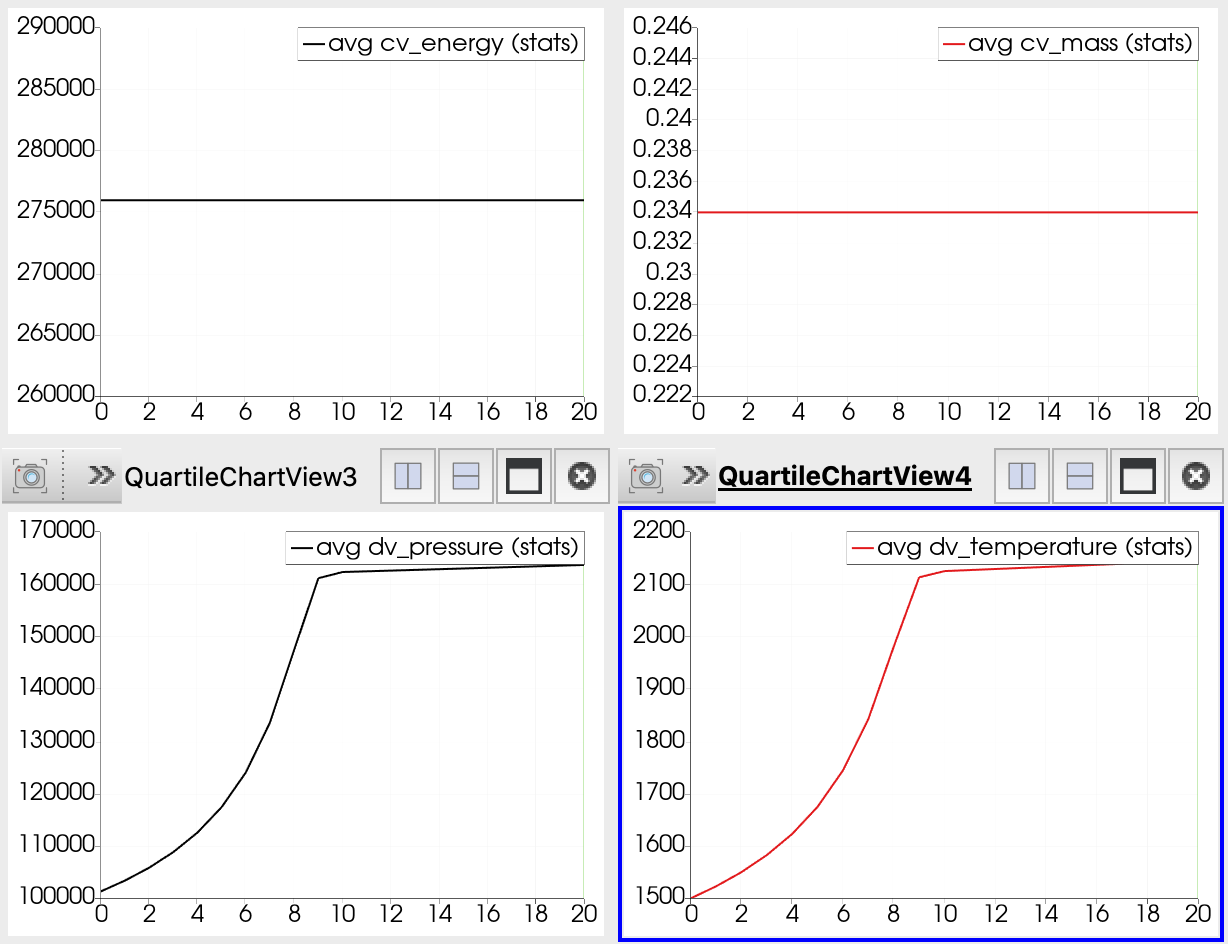
\includegraphics[width=.5\textwidth]{figures/mtc/autoignition_data_raw.png}
%     \end{multicols}
%\end{frame}


\begin{frame}\frametitle{\textit{Pyrometheus} in \textit{MIRGE-Euler}}
  \begin{multicols}{2}
    Governing equation is Navier--Stokes:
    \begin{equation*}
      \frac{\partial\mathbf{Q}}{\partial{t}} + \nabla \cdot (\mathbf{F}^I - \mathbf{F}^V) - \mathbf{S} = 0
    \end{equation*}
    With chemistry source terms:
    \begin{equation*}
      \mathbf{S} = [ 0, 0, 0, 0, 0, W_k\dot{\omega_k} ]
    \end{equation*}
    Thermo state functions:
    \begin{equation*}
      (p, T, e_k) = f(\mathbf{Q})
    \end{equation*}
    \begin{center}
      \prj{\tiny}{\textit{Prometheus} documentation}
    \end{center}
    \columnbreak
    % \lstinputlisting[style=kkcodestyle, basicstyle=\tiny, language=Python]{figures/mtc/chemsrc.py}
  \end{multicols}
\end{frame}

\begin{frame}\frametitle{Autoignition using \textit{MIRGE-Euler}}
  \begin{multicols}{2}
    \begin{itemize}
      \item Ethylene, oxygen mixture $\phi=1$, fixed $\rho$
      \item $(p, T) = (1 \mathtt{atm}, 1500 \mathtt{K})$
      \item \textit{Prometheus}-predicted profiles match \textit{Cantera}
      \item \textit{MIRGE-Euler} co-verification w/\textit{Pyrometheus} EOS
    \end{itemize}
  \end{multicols}
  \begin{multicols}{2}
    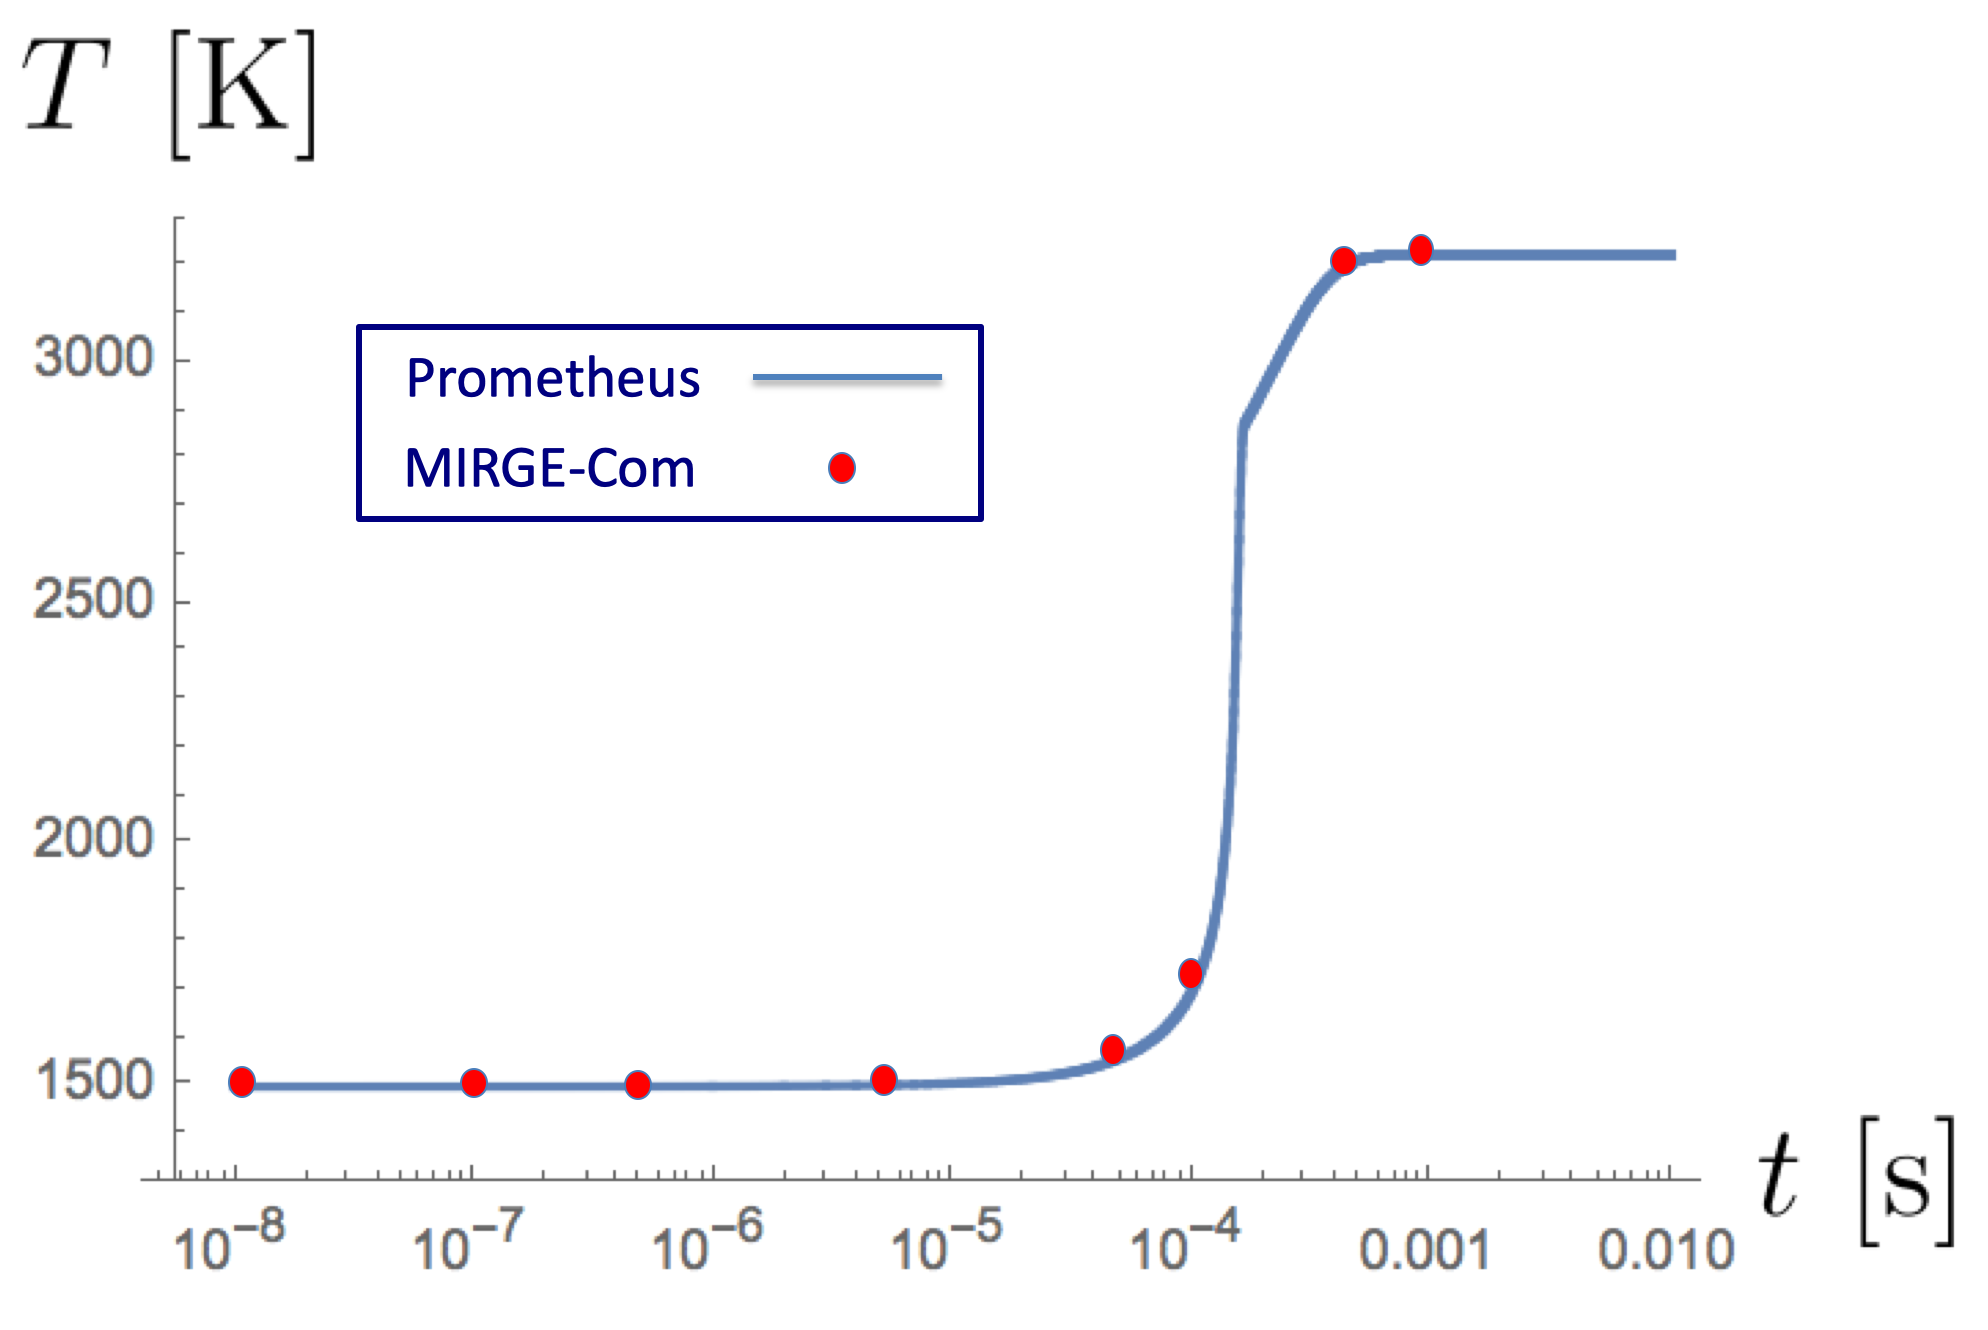
\includegraphics[width=.5\textwidth]{figures/mtc/AutoIgnition_Sudden.png}\\
    \columnbreak
    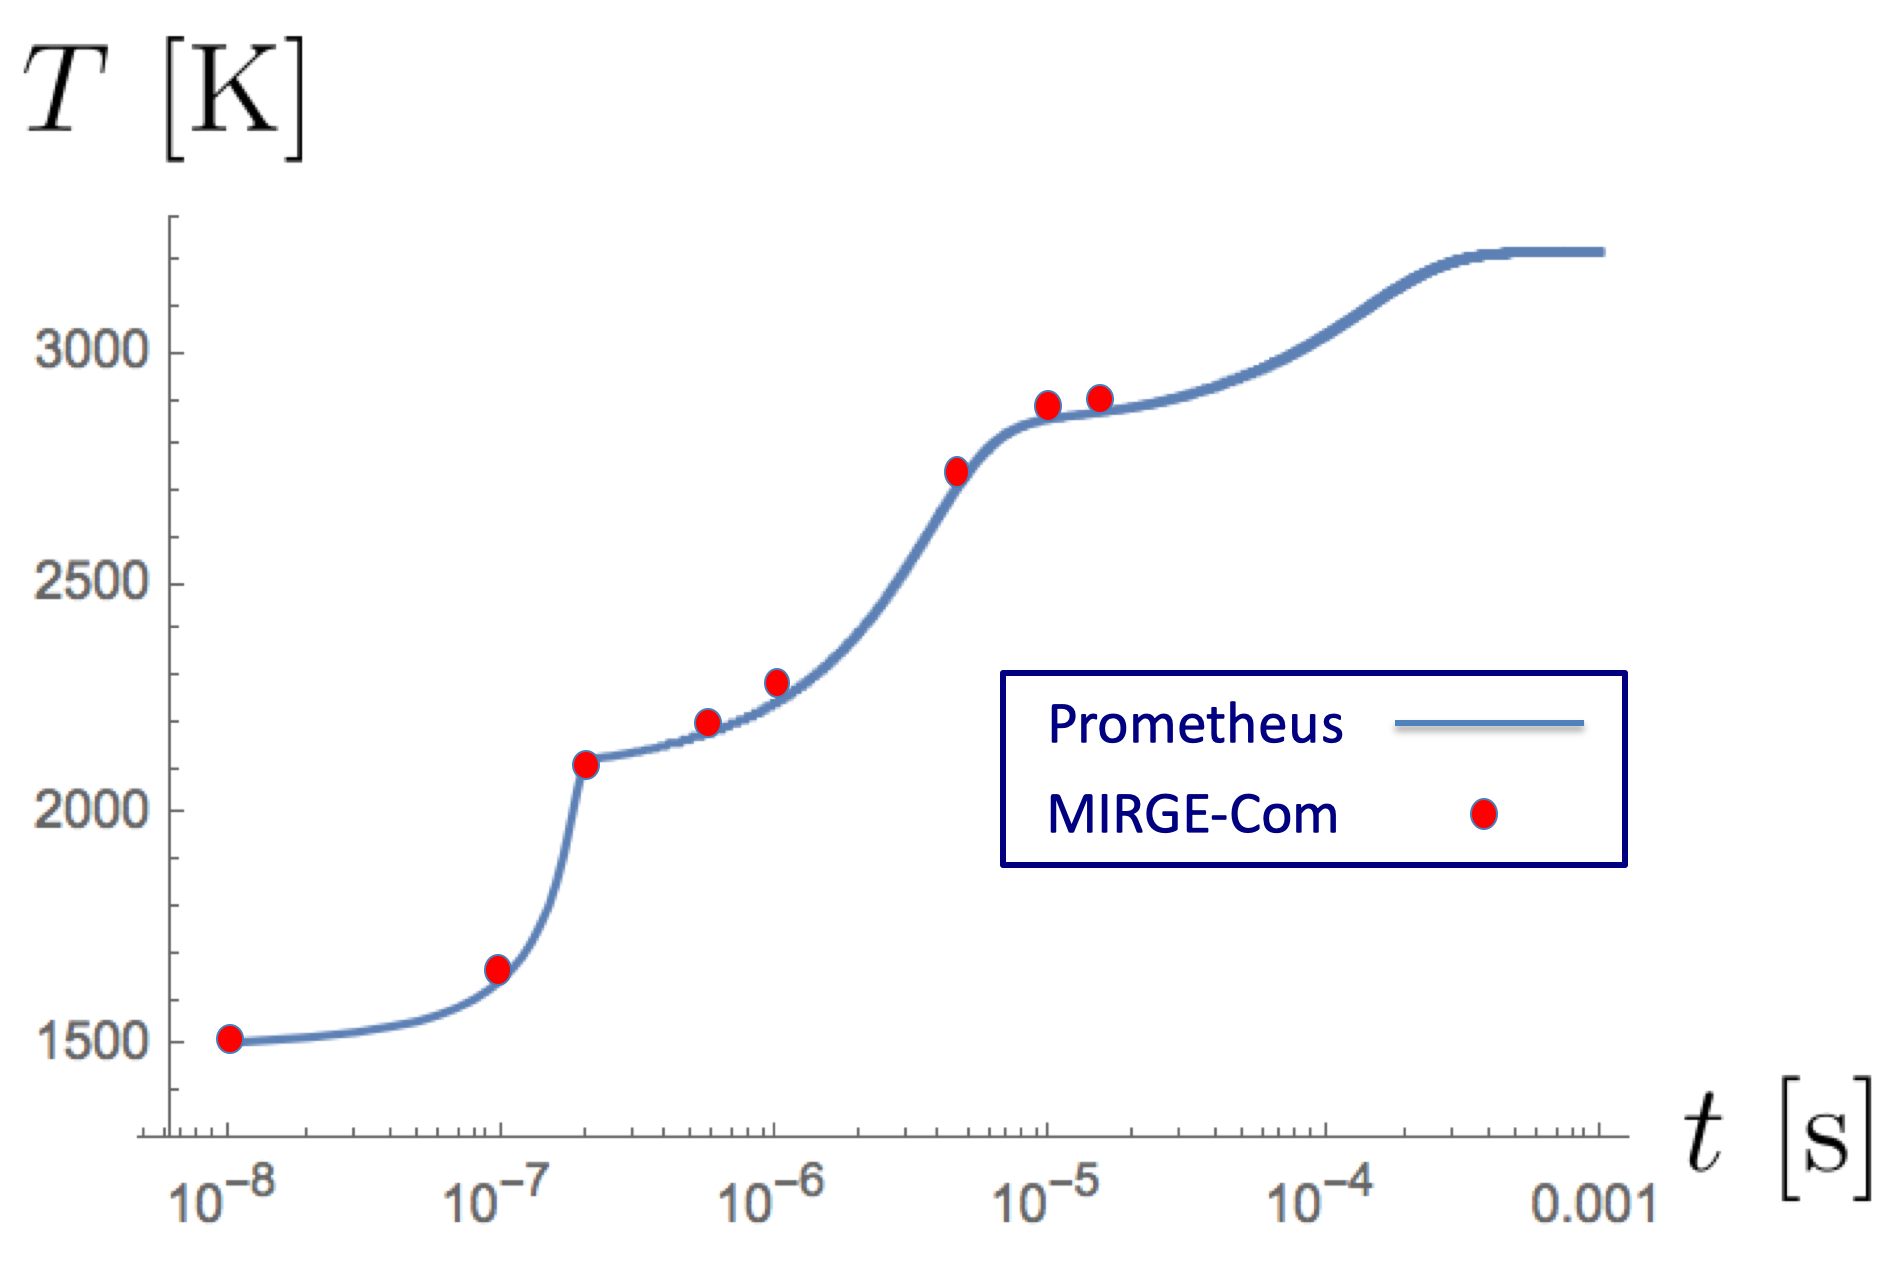
\includegraphics[width=.5\textwidth]{figures/mtc/AutoIgnition_Episodic.png}
  \end{multicols}
\end{frame}

\begin{frame}\frametitle{Retrospection \& path forward}
  \begin{multicols}{2}
    \begin{itemize}
    \item Awesome
      \begin{itemize}
        % PROS
        % 
        % - GPUs, MPI, DG
        % Very easy to go from concept and model to working simulation
      \item Follow the rules, everything works great! (GPU, MPI, DG)
      \item Easy to go from concept/model to working sim application
      \item Quite easy to read and understand 
      \item Close to the symbolic expressions
      \end{itemize}
      \columnbreak
    \item Troublesome
      \begin{itemize}
      \item Discovering the rules can be challenging
      \item Fixing things once you've run afoul of the rules
      \item Data structures are multi-faceted and can be confusing
      \item Performance is concerning
      \end{itemize}
    \end{itemize}
  \end{multicols}
  % Far more excited than frightened!
  \begin{center}
    Next for \textit{MIRGE-Com}
  \end{center}
  \begin{multicols}{2}
    \begin{itemize}
    \item Performance evaluation \& analysis \prj{\tiny}{M.~Diener}
    \item Viscous terms / Navier--Stokes / Diffusion
    \item Shock capturing \prj{\tiny}{Wyatt Hagen}
    \item Wall modeling / coupling \prj{\tiny}{M.~Smith}
    \item Post-diction in-tandem! \prj{\tiny}{M.~Anderson}
    \end{itemize}
  \end{multicols}
\end{frame}



%======================================================================
%\begin{frame}\frametitle{MIRGECom status and developments}
%  \begin{center}
%    Outline
%  \end{center}
%  \begin{itemize}
%  % MIRGE (Com) and how it is constructed, how it comes together
%  \item High-level architecture
%    
%  \item Navier-Stokes w/mixtures \& wall cartoon
%    \begin{itemize}
%    \item highlight current \& to come (Wyatt - shock capt, MattS - wall model, Esteban - thermochem kinetics)
%    \item show example code expressions for NS
%    % How prometheus connects
%    \item show Pyrometheus integration plan (and how is currently implemented)
%    \end{itemize}
%  \item MIRGE-Euler example(s):
%    \begin{itemize}
%    \item Building a driver
%    \item Brief about I/O \& analysis (maybe in arch overview?)
%    \item Autoignition example 
%    \item Allude to MikeA's Y0 sim
%    \end{itemize}
%  \end{itemize}
%\end{frame}
%======================================================================

%\begin{frame}\frametitle{Core packages}
%\begin{itemize}
%  \item Loo.py (\href{https://github.com/inducer/loopy}{(\textcolor{blue}{https://github.com/inducer/loopy})})
%  \begin{itemize}
%    \item Code generator and transform tool
%    \item IR in MIRGE
%    \item Element-wise computational kernels
%  \end{itemize}
%  \item Meshmode (\href{https://github.com/inducer/meshmode}{(\textcolor{blue}{https://github.com/inducer/meshmode})})
%  \begin{itemize}
%    \item Uns., high-order, discont. piecewise polynomial discretizations 
%    \item DG building blocks (see \texttt{examples/simple-dg.py}).
%  \end{itemize}
%  \item \textit{Grudge} - 1/2/3D DG based on \textit{meshmode} (\href{https://github.com/inducer/grudge}{(\textcolor{blue}{https://github.com/inducer/grudge})})
%  \begin{itemize}
%    \item Multiple \textit{meshmode} discretizations
%    \item Methods and operations - math, projections, norms and reductions
%  \end{itemize}
%\end{itemize}
%\end{frame}

%\begin{frame}\frametitle{Development team}
%\begin{multicols}{2}
%\begin{itemize}
%\item Mike Anderson - predictions, modeling
%\item Mike Campbell - sim/solver development
%\columnbreak
%\item Matthias Diener - environment, platforms, performance
%\item Matt Smith  - sim/solver development, grids/geometry
%\end{itemize}
%\end{multicols}
%\end{frame}

%\begin{frame}\frametitle{Target problem}
%  \begin{itemize}
%  \item Domain cartoon
%    % MIRGE (Com) and how it is constructed, how it comes together
%  \item Navier-Stokes w/mixtures \& chemical sources for fluid \& wall cartoon
%  \item Wall and viscous fluxes - Matt Smith heat eqn solver
%  \item Inviscid part - expressions for fluxes, implementation
%  \item Chemistry, Pyrometheus - Esteban
%    \begin{itemize}
%    \item architecture plug here \& generator use to generate python
%    \item expression for sources, implementation
%    \end{itemize}
%  \item Shock-capturing - Wyatt Hagen
%  \end{itemize}
%\end{frame}

%\begin{frame}\frametitle{User experience}
%  \begin{itemize}
%  \item Problem setup
%    \begin{itemize}
%    \item Grid - generate or read in (M. Smith hook)
%    \item Building a driver
%    \item Brief about I/O \& analysis (maybe in arch overview?)
%    \end{itemize}
%  \item Example drivers
%    \begin{itemize}
%    \item Isentropic vortex verif
%    \item Autoignition example 
%    \item Allude to MikeA's Y0 sim
%    \end{itemize}
%  \end{itemize}
%\end{frame}

%\begin{frame}\frametitle{High-level architecture}
%\end{frame}

%\begin{frame}\frametitle{Getting started with \textit{MIRGE-Com}}
%\begin{multicols}{2}
%\begin{itemize}
%  \item \textit{Emirge} - \textit{MIRGE-Com} installation tool
%  \begin{itemize}
%    \item > git clone https://github.com/illinois-ceesd/emirge
%    \item > install.sh
%    \item > source config/activate\_env.sh
%  \end{itemize}
%  \item \textit{MIRGE-Com} documentation
%  \begin{itemize}
%    \item > conda install sphinx
%    \item > cd mirgecom/doc \&\& make html
%  \end{itemize}
%\end{itemize}
%%\hspace{.8in}
%%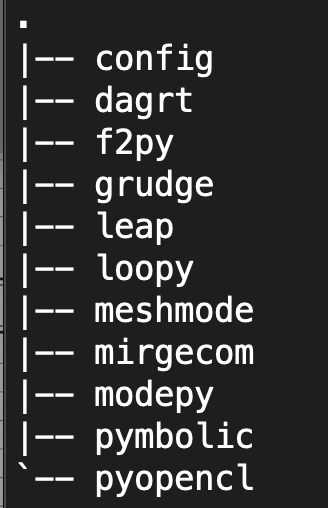
\includegraphics[width=.2\textwidth]{figures/mtc/emirge_dirs.png}
%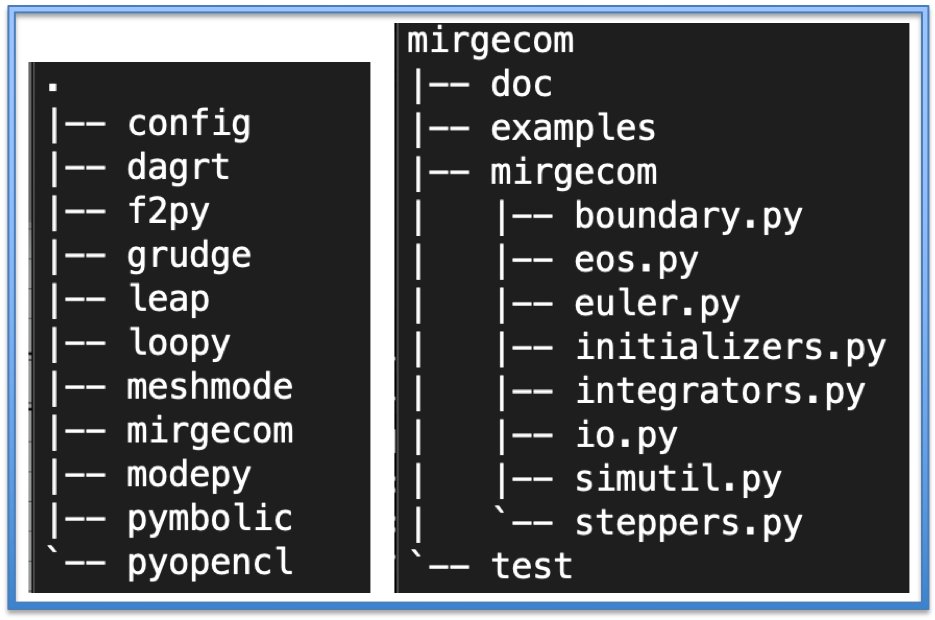
\includegraphics[width=.5\textwidth]{figures/mtc/dir_trees.png}
%\end{multicols}
%\begin{center}
%\href{https://github.com/illinois-ceesd/emirge}{(\textcolor{blue}{https://github.com/illinois-ceesd/emirge})}
%\href{https://mirgecom.readthedocs.io/en/latest/}{(\textcolor{blue}{https://mirgecom.readthedocs.io/en/latest/})}
%\end{center}
%\end{frame}


%\begin{frame}\frametitle{DG Support - Sub-discretizations (dd)}
%  \begin{multicols}{2}
%    \begin{itemize}
%    \item Projections between sub-discretizations: ``vol'' $\rightarrow$ ``int\_faces''
%    \end{itemize}
%    \lstinputlisting[style=kkcodestyle, basicstyle=\scriptsize, language=Python]{figures/mtc/project_sample.py}
%    \columnbreak
%    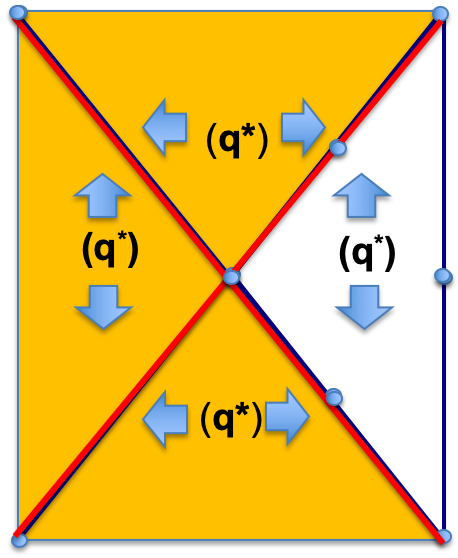
\includegraphics[width=.5\textwidth]{figures/mtc/grid_cartoon_6.png}
%  \end{multicols}
%\end{frame}

%\begin{frame}\frametitle{DG Support - Sub-discretizations (dd)}
%  \begin{multicols}{2}
%    \begin{itemize}
%    \item Unit normal to sub-discretizations
%    \end{itemize}
%    \lstinputlisting[style=kkcodestyle, basicstyle=\scriptsize, language=Python]{figures/mtc/normal_sample.py}
%    \columnbreak
%    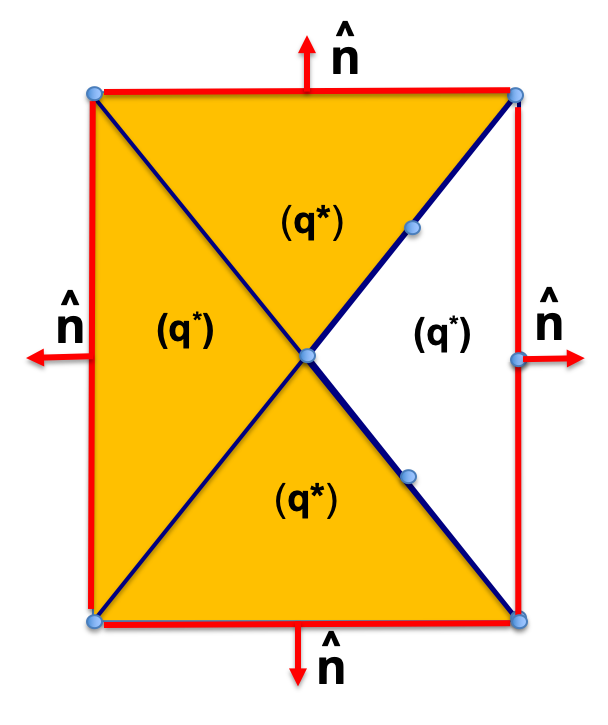
\includegraphics[width=.5\textwidth]{figures/mtc/grid_cartoon_normals.png}
%    %    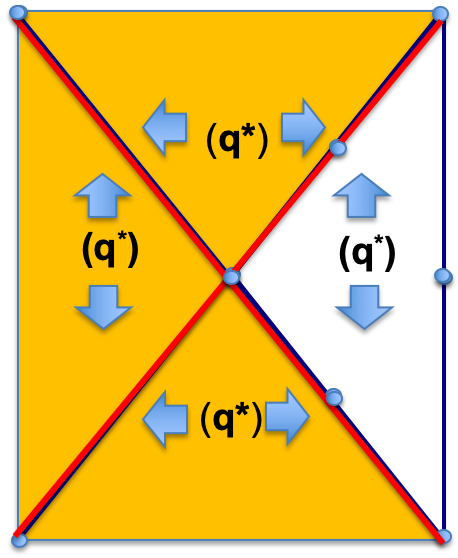
\includegraphics[width=.5\textwidth]{figures/mtc/grid_cartoon_6.png}
%  \end{multicols}
%\end{frame}

%\begin{frame}\frametitle{DG Support - Sub-discretizations (dd)}
%  \begin{multicols}{2}
%    \begin{itemize}
%    \item \textit{Grudge} TracePair data structure for element boundary data
%    \end{itemize}
%% *    \inputminted[mathescape,xleftmargin=0.2in]{python}{figures/mtc/tracepair_sample.py}
%    \columnbreak
%    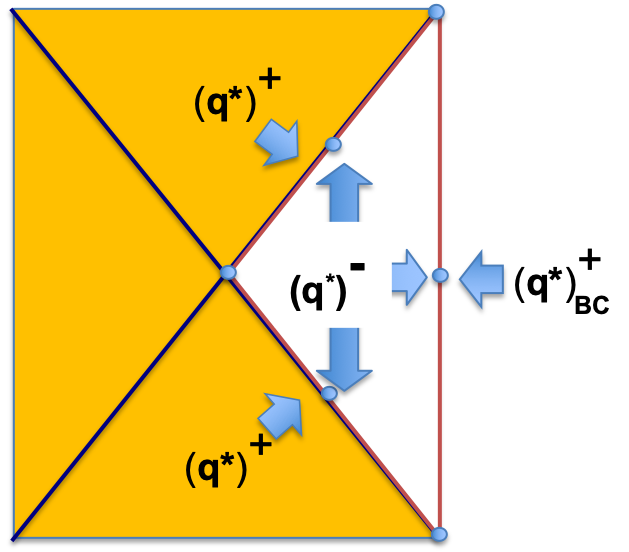
\includegraphics[width=.5\textwidth]{figures/mtc/tracepair_data_cartoon.png}
%  \end{multicols}
%\end{frame}

%\begin{frame}\frametitle{DG Support - Sub-discretizations (dd)}
%  \begin{multicols}{2}
%    \begin{itemize}
%    \item Projections between sub-discretizations: ``vol'' $\rightarrow$ ``int\_faces''
%    \end{itemize}
%    \begin{minted}{python}
%      discr.project("vol", "all_faces", q) 
%    \end{minted}
%    \begin{itemize}
%    \end{itemize}
%    
%    \columnbreak
%    %    %\begin{center}
%    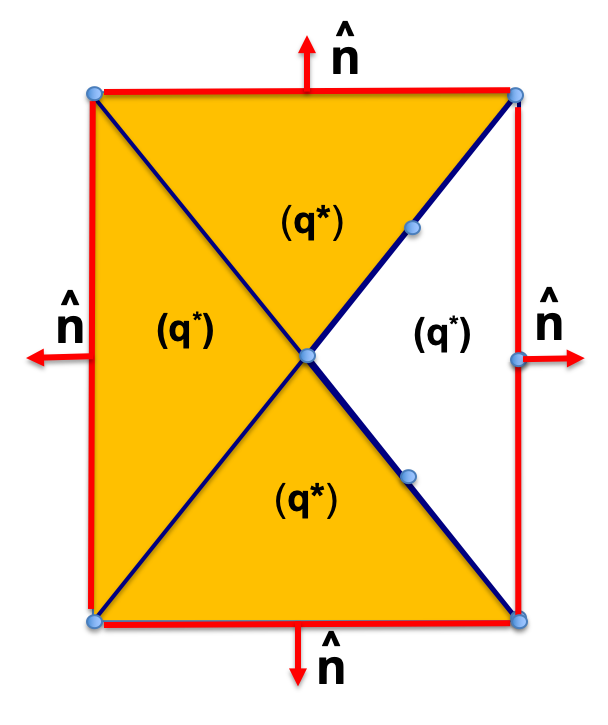
\includegraphics[width=.5\textwidth]{figures/mtc/grid_cartoon_normals.png}
%%    %\end{center}
%  \end{multicols}
%\end{frame}

%\begin{frame}\frametitle{DG Support}
% \begin{multicols}{2}
%\begin{center}
%  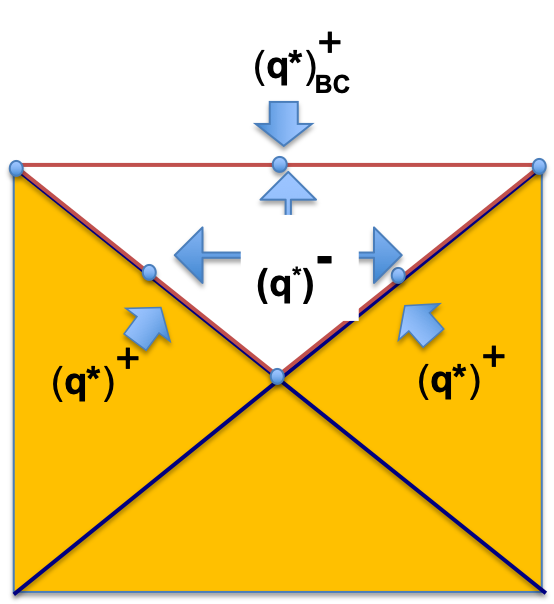
\includegraphics[width=.5\textwidth]{figures/mtc/tracepair_boundaries.png}
%\end{center}
%\end{multicols}
%\end{frame}

% CONS
% Datastructures are a little tough to figure out
% Python - and how it acts on the data structures
% Running afoul of the rules is easy - requires experience
% - some deeper documentation is lacking
% - too hard to discover the rules
% Adding your own kernel C/F90 --> MIRGE
% - mysterious
% Scaling and performance are challenging
%
% PROS
% Follow the rules, and everything works great
% - GPUs, MPI, DG
% Very easy to go from concept and model to working simulation
